%
% jacobi.tex
%
% (c) 2021 Prof Dr Andreas Müller, OST Ostschweizer Fachhochschule
%
\section{Jacobische elliptische Funktionen
\label{buch:elliptisch:section:jacobi}}
\rhead{Jacobische elliptische Funktionen}
Die elliptischen Integrale von
Abschnitt~\ref{buch:elliptisch:section:integral}
können dazu verwendet werden, die Länge eines Ellipsenbogens aus
den Koordinaten der Endpunkte zu berechnen.
Die trigonometrischen Funktionen drücken dagegen umgekehrt die
Koordinaten eines Punktes auf einem Kreis aus der Länge des
Kreisbogens aus.
Das elliptische Integral, welches die Bogenlänge auf einer Ellipse zwischen
den Punkten $(1,0)$ und $(x,y)$ entsprecht also eher der Funktion
$\arcsin y=\sin^{-1}y$.
Möchte man Funktionen konstruieren, die die Eigenschaften der 
trigonometrischen Funktionen auf die Geometrie von Ellipsen erweitern,
dann muss man die Umkehrfunktionen der elliptischen Integrale dafür ins
Auge fassen.


\subsection{Elliptische Funktionen als Trigonometrie}
\begin{figure}
\centering
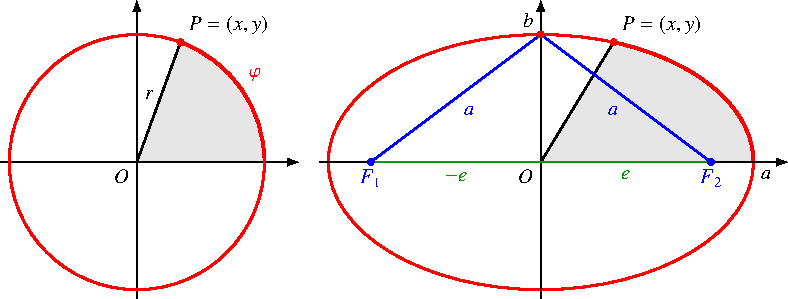
\includegraphics{chapters/110-elliptisch/images/ellipse.pdf}
\caption{Kreis und Ellipse zum Vergleich und zur Herleitung der 
elliptischen Funktionen von Jacobi als ``trigonometrische'' Funktionen
auf einer Ellipse.
\label{buch:elliptisch:fig:ellipse}}
\end{figure}
% based on Willliam Schwalm, Elliptic functions and elliptic integrals

\subsubsection{Geometrie einer Ellipse}
Eine {\em Ellipse} ist die Menge der Punkte der Ebene, für die die Summe
\index{Ellipse}%
der Entfernungen von zwei festen Punkten $F_1$ und $F_2$,
den {\em Brennpunkten}, konstant ist.
\index{Brennpunkt}%
In Abbildung~\ref{buch:elliptisch:fig:ellipse} eine Ellipse
mit Brennpunkten in $F_1=(-e,0)$ und $F_2=(e,0)$ dargestellt,
die durch die Punkte $(\pm a,0)$ und $(0,\pm b)$ auf den Achsen geht.
Der Punkt $(a,0)$ hat die Entfernungen $a+e$ und $a-e$ von den beiden
Brennpunkten, also die Entfernungssumme $a+e+a-e=2a$.
Jeder andere Punkt auf der Ellipse muss ebenfalls diese Entfernungssumme
haben, insbesondere auch der Punkt $(0,b)$.
Seine Entfernung zu jedem Brennpunkt muss aus Symmetriegründen gleich gross,
also $a$ sein.
Aus dem Satz von Pythagoras liest man daher ab, dass
\[
b^2+e^2=a^2
\qquad\Rightarrow\qquad
e^2 = a^2-b^2
\]
sein muss.
Die Strecke $e$ heisst auch {\em (lineare) Exzentrizität} der Ellipse.
Das Verhältnis $\varepsilon= e/a$  heisst die {\em numerische Exzentrizität}
der Ellipse.

\subsubsection{Ellipsengleichung}
Der Punkt $P=(x,y)$ auf der Ellipse hat die Entfernungen
\begin{equation}
\begin{aligned}
\overline{PF_1}^2
&=
y^2 + (x+e)^2
\\
\overline{PF_2}^2
&=
y^2 + (x-e)^2
\end{aligned}
\label{buch:elliptisch:eqn:wurzelausdruecke}
\end{equation}
von den Brennpunkten, für die 
\begin{equation}
\overline{PF_1}+\overline{PF_2}
=
2a
\label{buch:elliptisch:eqn:pf1pf2a}
\end{equation}
gelten muss.
Man kann nachrechnen, dass ein Punkt $P$, der die Gleichung
\[
\frac{x^2}{a^2} + \frac{y^2}{b^2}=1
\]
erfüllt, auch die Eigenschaft~\eqref{buch:elliptisch:eqn:pf1pf2a}
erfüllt.
Zur Vereinfachung setzen wir $l_1=\overline{PF_1}$ und $l_2=\overline{PF_2}$.
$l_1$ und $l_2$ sind Wurzeln aus der rechten Seite von
\eqref{buch:elliptisch:eqn:wurzelausdruecke}.
Das Quadrat von $l_1+l_2$ ist
\[
l_1^2 + 2l_1l_2 + l_2^2 = 4a^2.
\]
Um die Wurzeln ganz zu eliminieren, bringt man das Produkt $l_1l_2$ alleine
auf die rechte Seite und quadriert.
Man muss also verifizieren, dass
\[
(l_1^2 + l_2^2 -4a^2)^2 = 4l_1^2l_2^2.
\]
In den entstehenden Ausdrücken muss man ausserdem $e=\sqrt{a^2-b^2}$ und
\[
y=b\sqrt{1-\frac{x^2}{a^2}}
\]
substituieren.
Diese Rechnung führt man am einfachsten mit Hilfe eines
Computeralgebraprogramms durch, welches obige Behauptung bestätigt.

\subsubsection{Normierung}
Die trigonometrischen Funktionen sind definiert als Verhältnisse 
von Seiten rechtwinkliger Dreiecke.
Dadurch, dass man den die Hypothenuse auf Länge $1$ normiert, 
kann man die Sinus- und Kosinus-Funktion als Koordinaten eines
Punktes auf dem Einheitskreis interpretieren.

Für die Koordinaten eines Punktes auf der Ellipse ist dies nicht so einfach,
weil es nicht nur eine Ellipse gibt, sondern für jede numerische Exzentrizität
mindestens eine mit Halbeachse $1$.
Wir wählen die Ellipsen so, dass $a$ die grosse Halbachse ist, also $a>b$.
Als Normierungsbedingung verwenden wir, dass $b=1$ sein soll.
Dann ist $a=1/\varepsilon>1$.
In dieser Normierung haben Punkte $(x,y)$ auf der Ellipse $y$-Koordinaten
zwischen $-1$ und $1$ und $x$-Koordinaten zwischen $-a$ und $a$.

Im Zusammenhang mit elliptischen Funktionen wird die numerische Exzentrizität
$\varepsilon$ auch mit
\[
k
=
\varepsilon
=
\frac{e}{a}
=
\frac{\sqrt{a^2-b^2}}{a}
=
\frac{\sqrt{a^2-1}}{a},
\]
die Zahl $k$ heisst auch der {\em Modulus}.
Man kann $a$ auch durch $k$ ausdrücken, durch quadrieren und umstellen
findet man
\[
k^2a^2 = a^2-1
\quad\Rightarrow\quad
1=a^2(k^2-1)
\quad\Rightarrow\quad
a=\frac{1}{\sqrt{k^2-1}}.
\]

Die Gleichung der ``Einheitsellipse'' zu diesem Modulus ist
\[
\frac{x^2}{a^2}+y^2=1
\qquad\text{oder}\qquad
x^2(k^2-1) + y^2 = 1.
\]

\subsubsection{Definition der elliptischen Funktionen}
Die elliptischen Funktionen für einen Punkt auf der Ellipse mit Modulus $k$
können jetzt als Verhältnisse der Koordinaten des Punktes definieren.
Es stellt sich aber die Frage, was man als Argument verwenden soll.
Es soll so etwas wie den Winkel $\varphi$ zwischen der $x$-Achse und dem
Radiusvektor zum Punkt $P$
darstellen, aber wir haben hier noch eine Wahlfreiheit, die wir später
ausnützen möchten.
Im Moment müssen wir die Frage noch nicht beantworten und nennen das
noch unbestimmte Argument $u$.
Wir kümmern uns später um die Frage, wie $u$ von $\varphi$ abhängt.

Die Funktionen, die wir definieren wollen, hängen ausserdem auch 
vom Modulus ab.
Falls der verwendete Modulus aus dem Zusammenhang klar ist, lassen
wir das $k$-Argument weg.

Die Punkte auf dem Einheitskreis haben alle den gleichen Abstand vom
Nullpunkt, dies ist gleichzeitig die definierende Gleichung $r^2=x^2+y^2=1$
des Kreises.
Die Punkte auf der Ellipse erfüllen die Gleichung $x^2/a^2+y^2=1$,
die Entfernung der Punkte $r=\sqrt{x^2+y^2}$ vom Nullpunkt variert aber.

In Analogie zu den trigonometrischen Funktionen setzen wir jetzt für 
die Funktionen
\[
\begin{aligned}
&\text{sinus amplitudinis:}&
\operatorname{sn}(u,k)&= y \\
&\text{cosinus amplitudinis:}&
\operatorname{cn}(u,k)&= \frac{x}{a} \\
&\text{delta amplitudinis:}&
\operatorname{dn}(u,k)&=\frac{r}{a}
\end{aligned}
\]
Aus der Gleichung der Ellipse folgt sofort, dass
\[
\operatorname{sn}(u,k)^2 + \operatorname{cn}(u,k)^2 = 1
\]
ist.
Der Satz von Pythagoras kann verwendet werden, um die Entfernung zu
berechnen, also gilt
\begin{equation}
r^2
=
a^2 \operatorname{dn}(u,k)^2
=
x^2 + y^2
=
a^2\operatorname{cn}(u,k)^2 + \operatorname{sn}(u,k)^2
\quad
\Rightarrow
\quad
a^2 \operatorname{dn}(u,k)^2
=
a^2\operatorname{cn}(u,k)^2 + \operatorname{sn}(u,k)^2.
\label{buch:elliptisch:eqn:sncndnrelation}
\end{equation}
Ersetzt man
$
a^2\operatorname{cn}(u,k)^2
=
a^2-a^2\operatorname{sn}(u,k)^2
$, ergibt sich
\[
a^2 \operatorname{dn}(u,k)^2
=
a^2-a^2\operatorname{sn}(u,k)^2
+
\operatorname{sn}(u,k)^2
\quad
\Rightarrow
\quad
\operatorname{dn}(u,k)^2
+
\frac{a^2-1}{a^2}\operatorname{sn}(u,k)^2
=
1,
\]
woraus sich die Identität
\[
\operatorname{dn}(u,k)^2 + k^2 \operatorname{sn}(u,k)^2 = 1
\]
ergibt.
Ebenso kann man aus~\eqref{buch:elliptisch:eqn:sncndnrelation}
die Funktion $\operatorname{cn}(u,k)$ eliminieren, was auf
\[
a^2\operatorname{dn}(u,k)^2
=
a^2\operatorname{cn}(u,k)^2
+1-\operatorname{cn}(u,k)^2
=
(a^2-1)\operatorname{cn}(u,k)^2
+1.
\]
Nach Division durch $a^2$ ergibt sich
\begin{align*}
\operatorname{dn}(u,k)^2
-
k^2\operatorname{cn}(u,k)^2
&=
\frac{1}{a^2}
=
\frac{a^2-a^2+1}{a^2}
=
1-k^2.
\end{align*}

\subsubsection{Ableitung}
Die trigonometrischen Funktionen sind deshalb so besonders nützlich 
für die Lösung von Schwingungsdifferentialgleichungen, weil sie die
Beziehungen
\[
\frac{d}{d\varphi}  \cos\varphi = -\sin\varphi
\qquad\text{und}\qquad
\frac{d}{d\varphi}  \sin\varphi = \cos\varphi
\]
erfüllen.
So einfach können die Beziehungen natürlich nicht sein, sonst würde sich
durch Integration ja wieder nur die trigonometrischen Funktionen ergeben.
Durch geschickte Wahl des Arguments $u$ kann man aber erreichen, dass
sie ähnlich nützliche Beziehungen zwischen den Ableitungen ergeben.

Gesucht ist jetzt also eine Wahl für das Argument $u$ zum Beispiel in
Abhängigkeit von $\varphi$, dass sich einfache und nützliche
Ableitungsformeln ergeben.
Wir setzen daher $u(\varphi)$ voraus und beachten, dass $x$ und $y$
ebenfalls von $\varphi$ abhängen, es ist
$y=\sin\varphi$ und $x=a\cos\varphi$.
Die Ableitungen von $x$ und $y$ nach $\varphi$ sind
\begin{align*}
\frac{dy}{d\varphi}
&=
\cos\varphi
=
\frac{1}{a} x
=
\operatorname{cn}(u,k)
\\
\frac{dx}{d\varphi}
&=
-a\sin\varphi
=
-a y
=
-a\operatorname{sn}(u,k).
\end{align*}
Daraus kann man jetzt die folgenden Ausdrücke für die Ableitungen der
elliptischen Funktionen nach $\varphi$ ableiten:
\begin{align*}
\frac{d}{d\varphi} \operatorname{sn}(u,z)
&=
\frac{d}{d\varphi} y(\varphi)
=
\cos\varphi
=
\frac{x}{a}
=
\operatorname{cn}(u,k)
&&\Rightarrow&
\frac{d}{du}
\operatorname{sn}(u,k)
&=
\operatorname{cn}(u,k) \frac{d\varphi}{du}
\\
\frac{d}{d\varphi} \operatorname{cn}(u,z)
&=
\frac{d}{d\varphi} \frac{x(\varphi)}{a}
=
-\sin\varphi
=
-\operatorname{sn}(u,k)
&&\Rightarrow&
\frac{d}{du}\operatorname{cn}(u,k)
&=
-\operatorname{sn}(u,k) \frac{d\varphi}{du}
\\
\frac{d}{d\varphi} \operatorname{dn}(u,z)
&=
\frac{x}{ar} \frac{dx}{d\varphi}
+
\frac{y}{ar} \frac{dy}{d\varphi}
\\
&=
\frac{x}{ar} (-a\operatorname{sn}(u,k))
+
\frac{y}{ar} \operatorname{cn}(u,k)
\\
&=
\frac{x}{ar}(-ay)
+
\frac{y}{ar} \frac{x}{a}
=
\frac{xy(-1+\frac{1}{a^2})}{r} 
\\
&=
-\frac{xy(a^2-1)}{a^2r} 
\\
&=
-\frac{a^2-1}{ar}
\operatorname{cn}(u,k) \operatorname{sn}(u,k)
\\
&=-k^2
\frac{a}{r}
\operatorname{cn}(u,k) \operatorname{sn}(u,k)
\\
&=
-k^2\frac{\operatorname{cn}(u,k)\operatorname{sn}(u,k)}{\operatorname{dn}(u,k)}
&&\Rightarrow&
\frac{d}{du} \operatorname{dn}(u,k)
&=
-k^2\frac{\operatorname{cn}(u,k)
\operatorname{sn}(u,k)}{\operatorname{dn}(u,k)}
\frac{d\varphi}{du}
\end{align*}
Die einfachsten Beziehungen ergeben sich offenbar, wenn man $u$ so
wählt, dass
\[
\frac{d\varphi}{du}
=
\operatorname{dn}(u,k)
=
\frac{r}{a}
\]
Damit haben wir die Ableitungsregeln
\begin{align*}
\frac{d}{du}\operatorname{sn}(u,k)
&=
\phantom{-}\operatorname{cn}(u,k)\operatorname{dn}(u,k)
\\
\frac{d}{du}\operatorname{cn}(u,k)
&=
-\operatorname{sn}(u,k)\operatorname{dn}(u,k)
\\
\frac{d}{du}\operatorname{dn}(u,k)
&=
-k^2\operatorname{sn}(u,k)\operatorname{cn}(u,k)
\end{align*}

XXX als elliptische Integrale \\
XXX algebraische Beziehungen \\
XXX Additionstheoreme \\
XXX Perioden
% use https://math.stackexchange.com/questions/3013692/how-to-show-that-jacobi-sine-function-is-doubly-periodic

\subsection{Elliptische Funktionen und elliptische Integrale}

XXX Ableitungen \\
XXX Werte \\

\subsection{Lösungen von Differentialgleichungen}
Die elliptischen Funktionen ermöglichen die Lösung gewisser nichtlinearer
Differentialgleichungen in geschlossener Form.
Ziel dieses Abschnitts ist, Differentialgleichungen der Form
\(
\ddot{x}(t)
=
p(x(t))
\)
mit einem Polynom dritten Grades als rechter Seite lösen zu können.

\subsubsection{Die Differentialgleichungen der elliptischen Funktionen}
Um Differentialgleichungen mit elliptischen Funktion lösen zu
können, muss man als erstes die Differentialgleichungen derselben
finden.
Quadriert man die Ableitungsregel für $\operatorname{sn}(u,k)$, erhält
man
\[
\biggl(\frac{d}{du}\operatorname{sn}(u,k)\biggr)^2
=
\operatorname{cn}(u,k)^2 \operatorname{dn}(u,k)^2.
\]
Die Funktionen auf der rechten Seite können durch $\operatorname{sn}(u,k)$
ausgedrückt werden.
\begin{align*}
\biggl(\frac{d}{du}\operatorname{sn}(u,k)\biggr)^2
&=
\biggl(
1-\operatorname{sn}(u,k)^2
\biggr)
\biggl(
1-k^2 \operatorname{sn}(u,k)^2
\biggr)
\\
&=
k^2\operatorname{sn}(u,k)^4 
-(1+k^2)
\operatorname{sn}(u,k)^2 
+1.
\end{align*}
Für die Funktion $\operatorname{cn}(u,k)$ ergibt analoge Rechnung
\begin{align*}
\frac{d}{du}\operatorname{cn}(u,k)
&=
-\operatorname{sn}(u,k) \operatorname{dn}(u,k)
\\
\biggl(\frac{d}{du}\operatorname{cn}(u,k)\biggr)^2
&=
\operatorname{sn}(u,k)^2 \operatorname{dn}(u,k)^2
\\
&=
\biggl(1-\operatorname{cn}(u,k)^2\biggr)
\biggl(1-k^2+k^2 \operatorname{cn}(u,k)^2\biggr)
\\
&=
-k^2\operatorname{cn}(u,k)^4
-
(1-k^2-k^2)\operatorname{cn}(u,k)^2
+
(1-k^2)
\\
\frac{d}{du}\operatorname{dn}(u,k)
&=
-k^2\operatorname{sn}(u,k)\operatorname{cn}(u,k)
\\
\biggl(
\frac{d}{du}\operatorname{dn}(u,k)
\biggr)^2
&=
\bigl(k^2 \operatorname{sn}(u,k)^2\bigr)
\bigl(k^2 \operatorname{cn}(u,k)^2\bigr)
\\
&=
\biggl(
1-\operatorname{dn}(u,k)^2
\biggr)
\biggl(
\operatorname{dn}(u,k)^2-k^2+1
\biggr)
\\
&=
-\operatorname{dn}(u,k)^4
-
2\operatorname{dn}(u,k)^2
-k^2+1.
\end{align*}
\begin{table}
\centering
\renewcommand{\arraystretch}{2}
\begin{tabular}{|>{$}l<{$}|>{$}l<{$}|>{$}c<{$}|>{$}c<{$}|>{$}c<{$}|>{$}c<{$}>{$}c<{$}>{$}c<{$}|}
\hline
\text{Funktion $y=$}&\text{Differentialgleichung}&\alpha&\beta&\gamma&\multicolumn{3}{c|}{Signatur}\\
\hline
\operatorname{sn}(u,k)
	& y'^2 = (1-y^2)(1-k^2y^2)
		&k^2&1&1 &+&+&+
\\
\operatorname{cn}(u,k)
	&y'^2 = (1-y^2)(1-k^2+k^2y^2)
		&-k^2	&2k^2-1&1-k^2 &-&&+
\\
\operatorname{dn}(u,k)
	& y'^2 = -(1-y^2)(1-k^2-y^2)
		&1	&1-k^2	&-(1-k^2)&+&+&-
\\
\hline
\end{tabular}
\caption{Elliptische Funktionen als Lösungsfunktionen für verschiedene
nichtlineare Differentialgleichungen der Art
\eqref{buch:elliptisch:eqn:1storderdglell}.
Die Vorzeichen der Koeffizienten $\alpha$, $\beta$ und $\gamma$
entscheidet darüber, welche Funktion für die Lösung verwendet werden
muss.
\label{buch:elliptisch:tabelle:loesungsfunktionen}}
\end{table}

Die elliptischen Funktionen genügen also alle einer nichtlinearen
Differentialgleichung erster derselben Art.
Das Quadrat der Ableitung ist ein Polynom vierten Grades der Funktion.
Um dies besser einzufangen, schreiben wir $\operatorname{zn}(u,k)$,
wenn wir eine beliebige der drei Funktionen
$\operatorname{sn}(u,k)$,
$\operatorname{cn}(u,k)$
oder
$\operatorname{dn}(u,k)$
meinen.
Die Funktion $\operatorname{zn}(u,k)$ ist also Lösung der
Differentialgleichung
\begin{equation}
\operatorname{zn}'(u,k)^2
=
\alpha \operatorname{zn}(u,k)^4 + \beta \operatorname{zn}(u,)^2 + \gamma,
\label{buch:elliptisch:eqn:1storderdglell}
\end{equation}
wobei wir mit $\operatorname{zn}'(u,k)$ die Ableitung von
$\operatorname{zn}(u,k)$ nach dem ersten Argument meinen.
Die Koeffizienten $\alpha$, $\beta$ und $\gamma$ hängen von $k$ ab,
vor allem aber haben Sie verschiedene Vorzeichen.
Je nach Vorzeichen sind also eine andere elliptische Funktion als
Lösung zu verwenden.


\subsubsection{Differentialgleichung zweiter Ordnung}
Leitet die Differentialgleichung ~\eqref{buch:elliptisch:eqn:1storderdglell}
man dies nochmals nach $u$ ab, erhält man die Differentialgleichung
\[
2\operatorname{zn}''(u,k)\operatorname{zn}'(u,k)
=
4\alpha \operatorname{zn}(u,k)^3\operatorname{zn}'(u,k) + 2\beta \operatorname{zn}'(u,k)\operatorname{zn}(u,k).
\]
Teilt man auf beiden Seiten durch $2\operatorname{zn}'(u,k)$,
bleibt die nichtlineare
Differentialgleichung
\[
\frac{d^2\operatorname{zn}}{du^2}
=
\beta \operatorname{zn} + 2\alpha \operatorname{zn}^3.
\]
Dies ist die Gleichung eines harmonischen Oszillators mit einer 
Anharmonizität der Form $2\alpha z^3$.

\subsubsection{Differentialgleichung des anharmonischen Oszillators}
Wir möchten die nichtlineare Differentialgleichung
\begin{equation}
\biggl(
\frac{dx}{dt}
\biggr)^2
=
Ax^4+Bx^2 + C
\label{buch:elliptisch:eqn:allgdgl}
\end{equation}
mit Hilfe elliptischer Funktionen lösen.
Wir nehmen also an, dass die gesuchte Lösung eine Funktion der Form
\begin{equation}
x(t) = a\operatorname{zn}(bt,k)
\label{buch:elliptisch:eqn:loesungsansatz}
\end{equation}
ist.
Die erste Ableitung von $x(t)$ ist
\[
\dot{x}(t) 
=
a\operatorname{zn}'(bt,k).
\]

Indem wir diesen Lösungsansatz in die
Differentialgleichung~\eqref{buch:elliptisch:eqn:allgdgl}
einsetzen, erhalten wir
\begin{equation}
a^2b^2 \operatorname{zn}'(bt,k)^2
=
a^4A\operatorname{zn}(bt,k)^4
+
a^2B\operatorname{zn}(bt,k)^2
+C
\label{buch:elliptisch:eqn:dglx}
\end{equation}
Andererseits wissen wir, dass $\operatorname{zn}(u,k)$ einer
Differentilgleichung der Form~\eqref{buch:elliptisch:eqn:1storderdglell}
erfüllt.
Wenn wir \eqref{buch:elliptisch:eqn:dglx} durch $a^2b^2$ teilen, können wir
die rechte Seite von \eqref{buch:elliptisch:eqn:dglx} mit der rechten
Seite von \eqref{buch:elliptisch:eqn:1storderdglell} vergleichen:
\[
\frac{a^2A}{b^2}\operatorname{zn}(bt,k)^4
+
\frac{B}{b^2}\operatorname{zn}(bt,k)^2
+\frac{C}{a^2b^2}
=
\alpha\operatorname{zn}(bt,k)^4
+
\beta\operatorname{zn}(bt,k)^2
+
\gamma\operatorname{zn}(bt,k).
\]
Daraus ergeben sich die Gleichungen
\begin{align}
\alpha &= \frac{a^2A}{b^2},
&
\beta &= \frac{B}{b^2}
&&\text{und}
&
\gamma &= \frac{C}{a^2b^2}
\label{buch:elliptisch:eqn:koeffvergl}
\intertext{oder aufgelöst nach den Koeffizienten der ursprünglichen
Differentialgleichung}
A&=\frac{\alpha b^2}{a^2}
&
B&=\beta b^2
&&\text{und}&
C &= \gamma a^2b^2
\label{buch:elliptisch:eqn:koeffABC}
\end{align}
für die Koeffizienten der Differentialgleichung der zu verwendenden
Funktion.

Man beachte, dass nach \eqref{buch:elliptisch:eqn:koeffvergl} die 
Koeffizienten $A$, $B$ und $C$ die gleichen Vorzeichen haben wie
$\alpha$, $\beta$ und $\gamma$, da in 
\eqref{buch:elliptisch:eqn:koeffvergl} nur mit Quadraten multipliziert
wird, die immer positiv sind.
Diese Vorzeichen bestimmen, welche der Funktionen gewählt werden muss.

In den Differentialgleichungen für die elliptischen Funktionen gibt
es nur den Parameter $k$, der angepasst werden kann.
Es folgt, dass die Gleichungen
\eqref{buch:elliptisch:eqn:koeffvergl} 
auch $a$ und $b$ bestimmen.
Zum Beispiel folgt aus der letzten Gleichung, dass
\[
b = \pm\sqrt{\frac{B}{\beta}}.
\]
Damit folgt dann aus der zweiten
\[
a=\pm\sqrt{\frac{\beta C}{\gamma B}}.
\]
Die verbleibende Gleichung legt $k$ fest.
Das folgende Beispiel illustriert das Vorgehen am Beispiel einer
Gleichung, die Lösungsfunktion $\operatorname{sn}(u,k)$ verlangt.

\begin{beispiel}
Wir nehmen an, dass die Vorzeichen von $A$, $B$ und $C$ gemäss
Tabelle~\ref{buch:elliptische:tabelle:loesungsfunktionen} verlangen,
dass die Funktion $\operatorname{sn}(u,k)$ für die Lösung verwendet
werden muss.
Die Tabelle sagt dann auch, dass 
$\alpha=k^2$, $\beta=1$ und $\gamma=1$ gewählt werden müssen.
Aus dem Koeffizientenvergleich~\eqref{buch:elliptisch:eqn:koeffvergl}
folgt dann der Reihe nach
\begin{align*}
b&=\pm \sqrt{B}
\\
a&=\pm \sqrt{\frac{C}{B}}
\\
k^2
&=
\frac{AC}{B^2}.
\end{align*}
Man beachte, dass man $k^2$ durch Einsetzen von
\eqref{buch:elliptisch:eqn:koeffABC}
auch direkt aus den Koeffizienten $\alpha$, $\beta$ und $\gamma$
erhalten kann, nämlich
\[
\frac{AC}{B^2}
=
\frac{\frac{\alpha b^2}{a^2} \gamma a^2b^2}{\beta^2 b^4}
=
\frac{\alpha\gamma}{\beta^2}.
\qedhere
\]
\end{beispiel}

Da alle Parameter im 
Lösungsansatz~\eqref{buch:elliptisch:eqn:loesungsansatz} bereits
festgelegt sind stellt sich die Frage, woher man einen weiteren
Parameter nehmen kann, mit dem Anfangsbedingungen erfüllen kann.
Die Differentialgleichung~\eqref{buch:elliptisch:eqn:allgdgl} ist
autonom, die Koeffizienten der rechten Seite der Differentialgleichung
sind nicht von der Zeit abhängig. 
Damit ist eine zeitverschobene Funktion $x(t-t_0)$ ebenfalls eine
Lösung der Differentialgleichung.
Die allgmeine Lösung der 
Differentialgleichung~\eqref{buch:elliptisch:eqn:allgdgl} hat
also die Form
\[
x(t) = a\operatorname{zn}(b(t-t_0)),
\]
wobei die Funktion $\operatorname{zn}(u,k)$ auf Grund der Vorzeichen
von $A$, $B$ und $C$ gewählt werden müssen.

\subsubsection{Das mathematische Pendel}
\begin{figure}
\centering
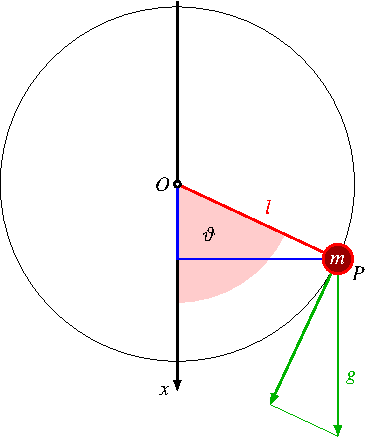
\includegraphics{chapters/110-elliptisch/images/pendel.pdf}
\caption{Mathematisches Pendel
\label{buch:elliptisch:fig:mathpendel}}
\end{figure}
Das in Abbildung~\ref{buch:elliptisch:fig:mathpendel} dargestellte
Mathematische Pendel besteht aus einem Massepunkt der Masse $m$
im Punkt $P$,
der über eine masselose Stange der Länge $l$ mit dem Drehpunkt $O$
verbunden ist.
Das Pendel bewegt sich unter dem Einfluss der Schwerebeschleunigung $g$.

Das Trägheitsmoment des Massepunktes um den Drehpunkt $O$ ist
\(
I=ml^2
\).
Das Drehmoment der Schwerkraft ist
\(M=gl\sin\vartheta\).
Die Bewegungsgleichung wird daher
\[
\begin{aligned}
\frac{d}{dt} I\dot{\vartheta}
&=
M
=
gl\sin\vartheta
\\
ml^2\ddot{\vartheta}
&=
gl\sin\vartheta
&&\Rightarrow&
\ddot{\vartheta}
&=\frac{g}{l}\sin\vartheta
\end{aligned}
\]
Dies ist eine nichtlineare Differentialgleichung zweiter Ordnung, die
wir nicht unmittelbar mit den Differentialgleichungen erster Ordnung
der elliptischen Funktionen vergleichen können.

Die Differentialgleichungen erster Ordnung der elliptischen Funktionen
enthalten das Quadrat der ersten Ableitung.
In unserem Fall entspricht das einer Gleichung, die $\dot{\vartheta}^2$
enthält.
Der Energieerhaltungssatz kann uns eine solche Gleichung geben.
Die Summe von kinetischer und potentieller Energie muss konstant sein.
Dies führt auf
\[
E_{\text{kinetisch}}
+
E_{\text{potentiell}}
=
\frac12I\dot{\vartheta}^2
+
mgl(1-\cos\vartheta)
=
\frac12ml^2\dot{\vartheta}^2
+
mgl(1-\cos\vartheta)
=
E
\]
Durch Auflösen nach $\dot{\vartheta}$ kann man jetzt die
Differentialgleichung
\[
\dot{\vartheta}^2
=
-
\frac{2g}{l}(1-\cos\vartheta)
+\frac{2E}{ml^2}
\]
finden.
In erster Näherung, d.h. wenn man die rechte Seite bis zu vierten
Potenzen in eine Taylor-Reihe in $\vartheta$ entwickelt,  ist dies
tatsächlich eine Differentialgleichung der Art, wie wir sie für
elliptische Funktionen gefunden haben, wir möchten aber eine exakte
Lösung konstruieren.

Wir verwenden als neue Variable 
\[
y = \sin\frac{\vartheta}2
\]
mit der Ableitung
\[
\dot{y}=\frac12\cos\frac{\vartheta}{2}\cdot \dot{\vartheta}.
\]
Man beachte, dass $y$ nicht eine Koordinate in
Abbildung~\ref{buch:elliptisch:fig:mathpendel} ist.

Aus den Halbwinkelformeln finden wir
\[
\cos\vartheta
=
1-2\sin^2 \frac{\vartheta}2
=
1-2y^2.
\]
Dies können wir zusammen mit der
Identität $\cos^2\vartheta/2 = 1-\sin^2\vartheta/2 = 1-y^2$
in die Energiegleichung einsetzen und erhalten
\[
\frac12ml^2\dot{\vartheta}^2 + mgly^2 = E.
\]
Durch Multiplizieren mit $\cos^2\frac{\vartheta}{2}=1-y^2$
erhalten wir auf der linken Seite einen Ausdruck, den wir
als Funktion von $\dot{y}$ ausdrücken können.
Wir erhalten
\begin{align*}
\frac12ml^2
\cos^2\frac{\vartheta}2
\dot{\vartheta}^2
&=
(1-y^2)
(E -mgly^2)
\\
\frac{1}{4}\cos^2\frac{\vartheta}{2}\dot{\vartheta}^2
&=
\frac{1}{2}
(1-y^2)
\biggl(\frac{E}{ml^2} -\frac{g}{l}y^2\biggr)
\\
\dot{y}^2
&=
\frac{E}{2ml^2}
(1-y^2)\biggl(
1-\frac{2gml}{E}y^2
\biggr).
\end{align*}
Dies ist genau die Form der Differentialgleichung für die elliptische
Funktion $\operatorname{sn}(u,k)$
mit $k^2 = gml/2E$.

XXX Differentialgleichung \\
XXX Mathematisches Pendel \\

\subsection{Soliton-Lösungen der Sinus-Gordon-Gleichung}

\subsection{Nichtlineare Differentialgleichung vierter Ordnung}
XXX Möbius-Transformation \\
XXX Reduktion auf die Differentialgleichung elliptischer Funktionen
